
\newpage

\section{Resultados e Análise de Dados}

\subsection{FPB}
O primeiro filtro projetado foi um filtro passa-baixas de terceira ordem, com 
resposta do tipo Butterworth utilizando apenas 1 indutor.

A figura \ref{fig:fpb-norm} mostra o circuito normalizado.
\begin{figure}[!h]
  \centering
  
  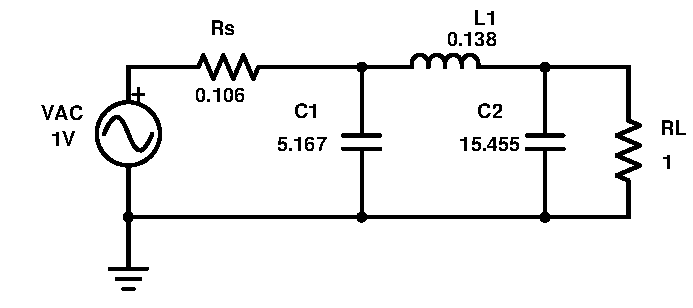
\includegraphics[scale=0.4]{Imagens/fpb-norm}
  \label{fig:fpb-norm}
  \caption{Filtro passa-baixas normalizado.}
\end{figure}


A figura \ref{fig:fpb} mostra o circuito já desnormalizado, pronto para 
simulação.
\begin{figure}[!h]
  \centering
  
  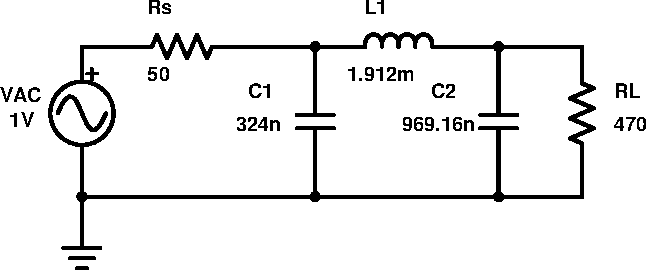
\includegraphics[scale=0.4]{Imagens/fpb}
  \label{fig:fpb}
  \caption{Filtro desnormalizado passa-baixas.}
\end{figure}

A resposta em frequência obtida está na figura \ref{fig:resp_freq}, onde foi 
obtido uma frequência de corte de 5,317 kHz. 

\begin{figure}[!h]
  \centering
  
  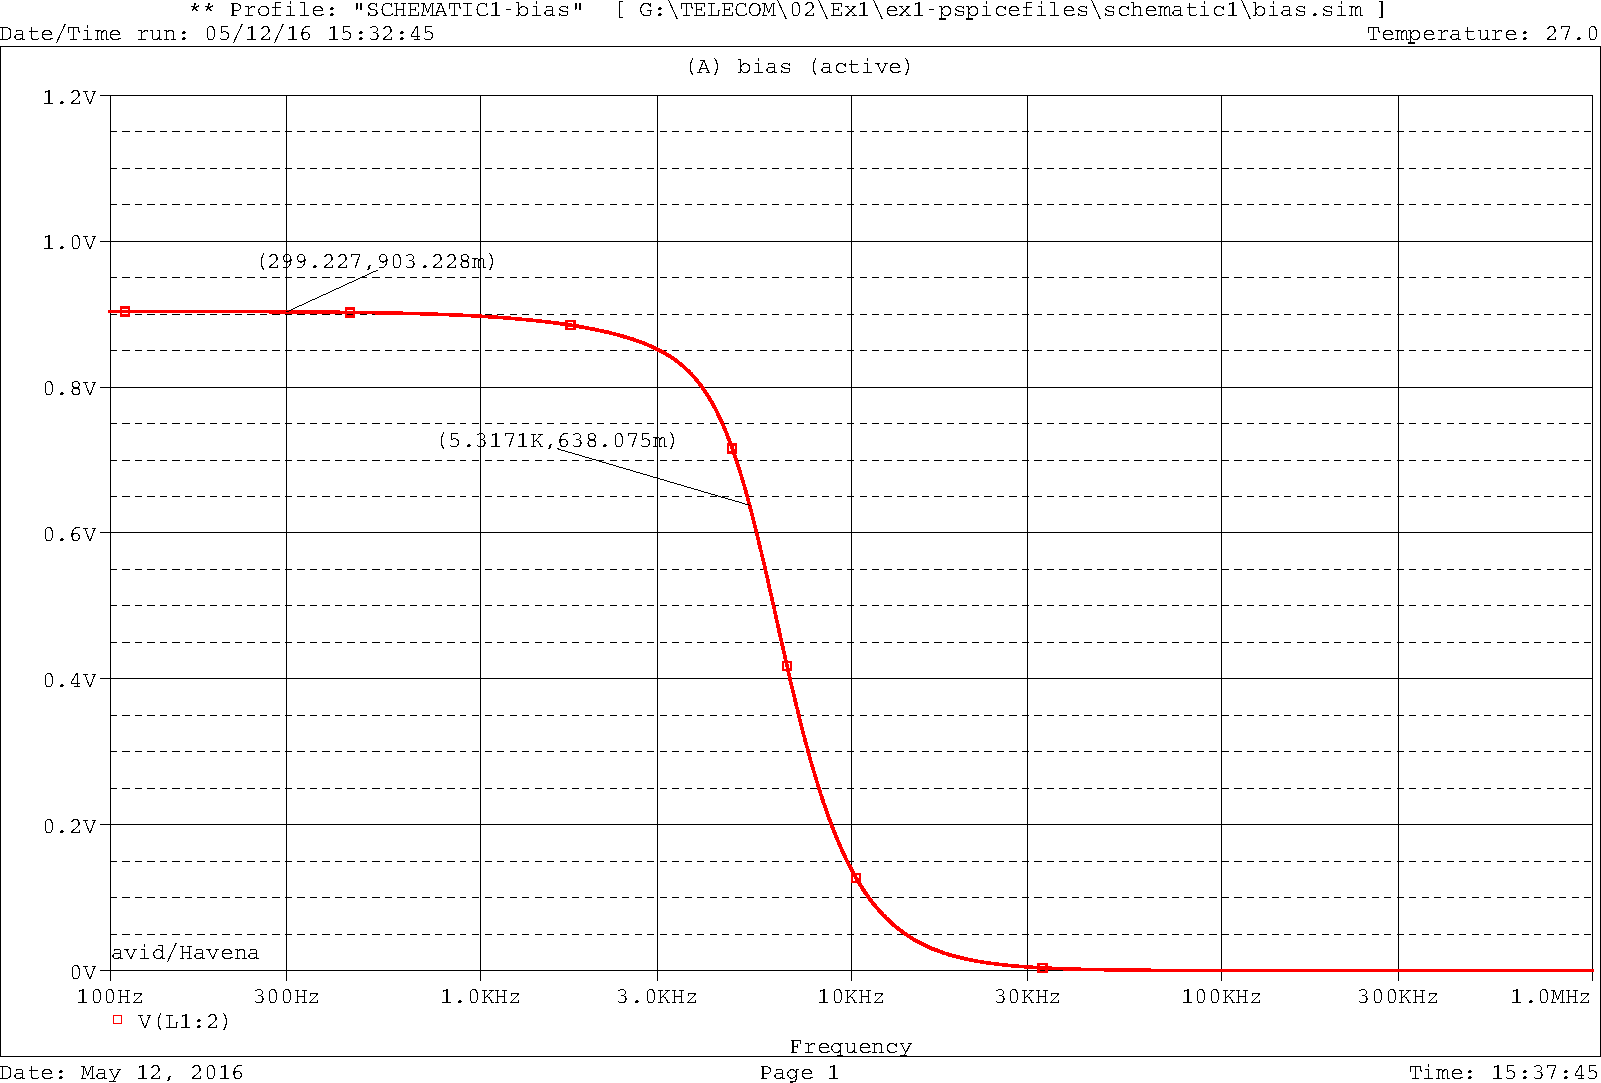
\includegraphics[scale=0.3]{Imagens/resp_freq}
  \label{fig:resp_freq}
  \caption{Resposta em frequência do filtro passa-baixas.}
\end{figure}

A figura \ref{fig:resp_freq_db} mostra a resposta em dB, nota-se que a 
atenuação aumenta em aproximadamente 60 dB por década, o que corresponde a 
ordem 3 do filtro.

\begin{figure}[!h]
  \centering
  
  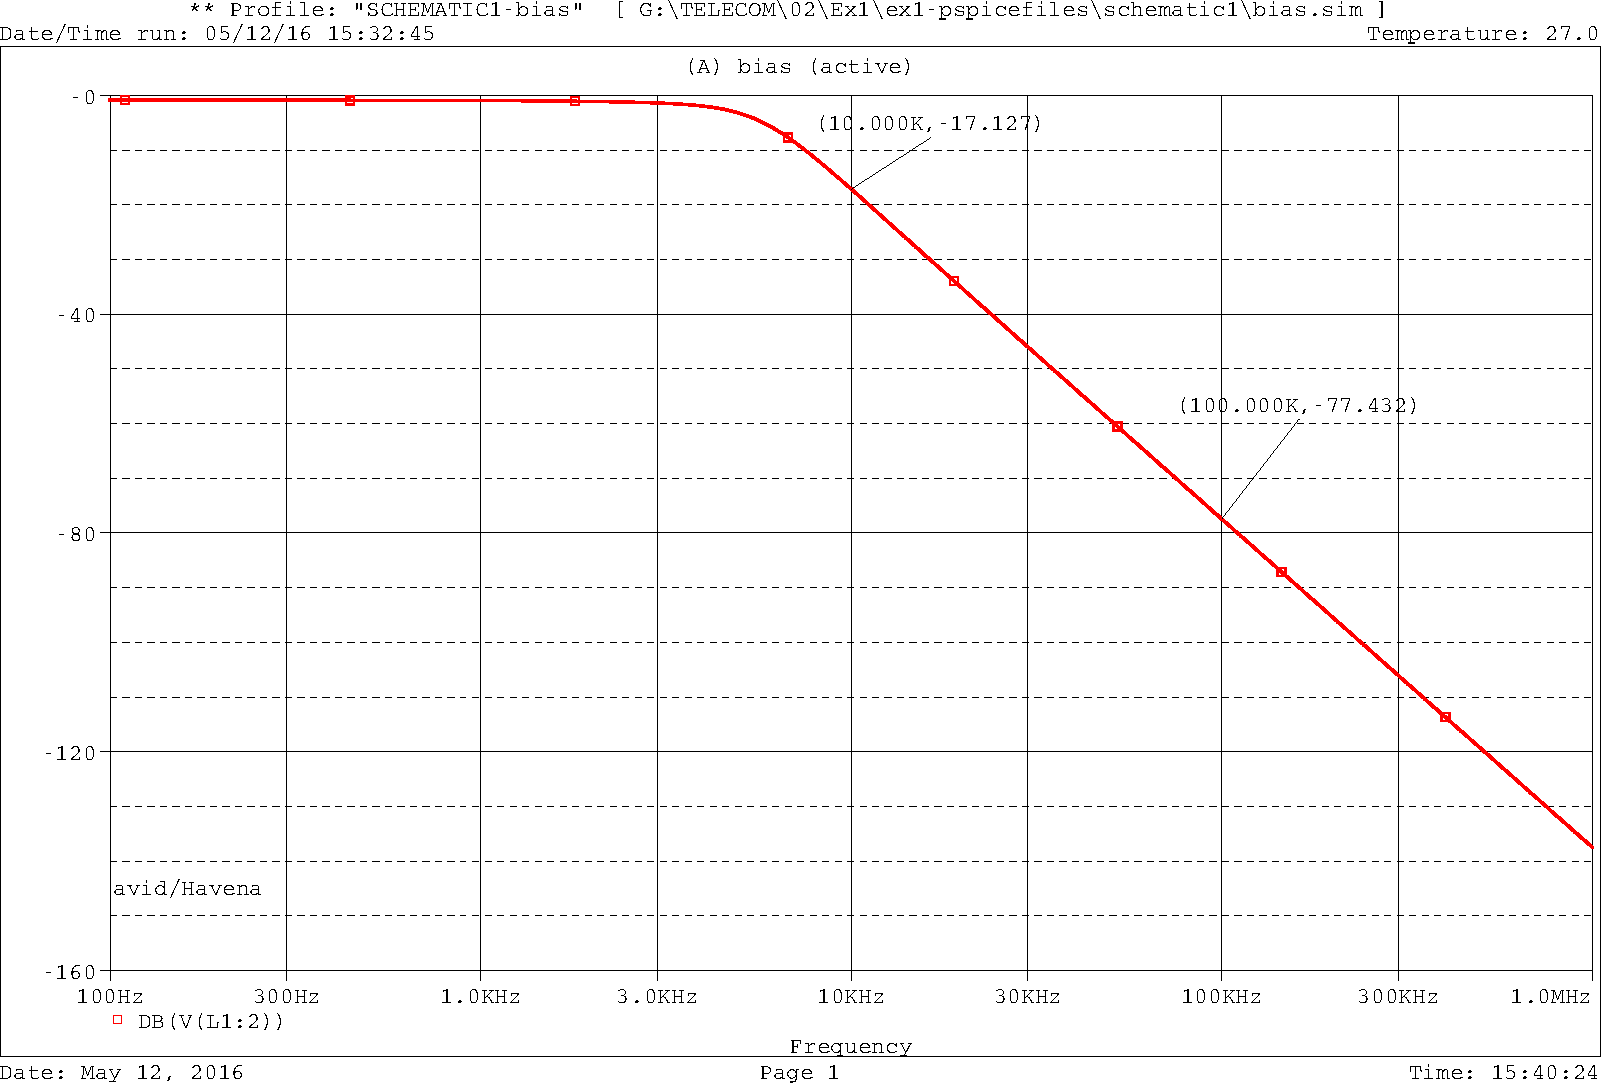
\includegraphics[scale=0.3]{Imagens/resp_freq_db}
  \label{fig:resp_freq_db}
  \caption{Resposta em frequência do filtro passa-baixas em dB.}
\end{figure}

A figura \ref{fig:resp_freq_phase} mostra a fase da resposta em frequência para 
o filtro passa baixas, onde é possível observar uma defasagem de 270 graus, o 
que condiz com a teoria pois o filtro é de ordem 3.

\begin{figure}[!h]
  \centering
  
  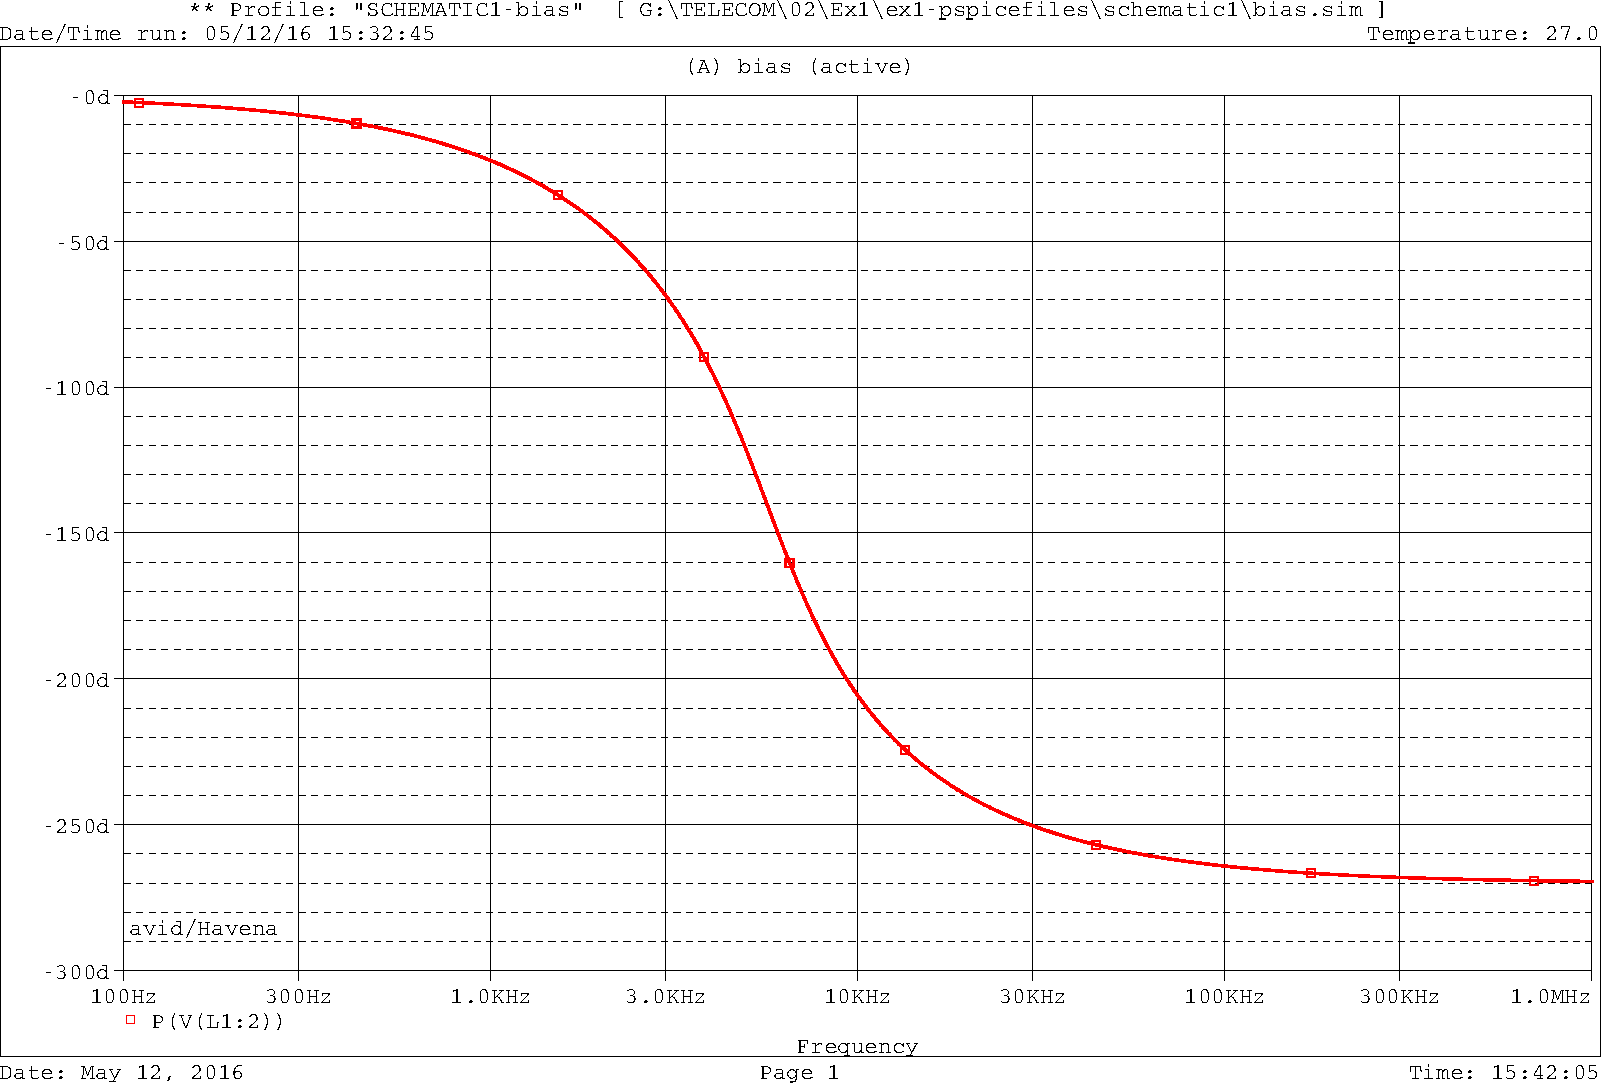
\includegraphics[scale=0.3]{Imagens/resp_freq_phase}
  \label{fig:resp_freq_phase}
  \caption{Fase da resposta em frequência do filtro passa-baixas.}
\end{figure}

\subsection{FPA}
O segundo filtro projetado foi um filtro passa-altas de terceira ordem, com 
resposta do tipo Butterworth utilizando apenas 1 indutor.

A figura \ref{fig:fpa-norm} mostra o circuito normalizado.
\begin{figure}[!h]
  \centering
  
  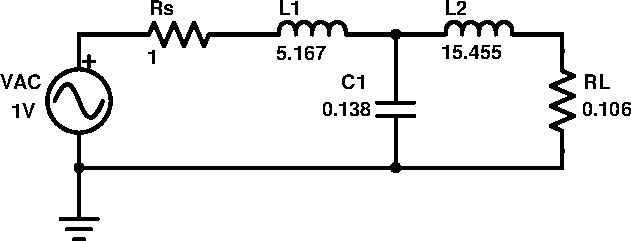
\includegraphics[scale=0.4]{Imagens/fpa-norm}
  \label{fig:fpa-norm}
  \caption{Filtro passa-altas normalizado.}
\end{figure}

A figura \ref{fig:fpa} mostra o circuito já desnormalizado, pronto para 
simulação.

\begin{figure}[!h]
  \centering
  
  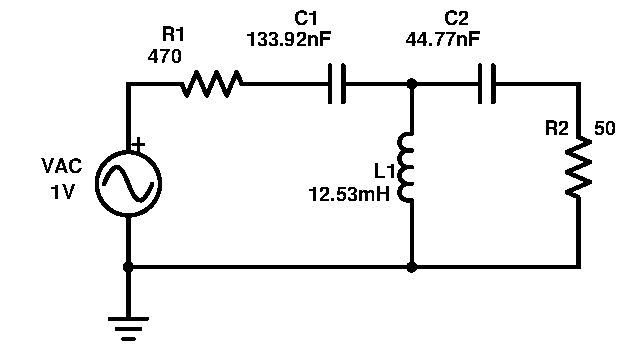
\includegraphics[scale=0.4]{Imagens/fpa}
  \label{fig:fpa}
  \caption{Filtro desnormalizado passa-altas.}
\end{figure}

A resposta em frequência obtida está na figura \ref{fig:resp_freq_2}, onde foi 
obtido uma frequência de corte de 4,384 kHz. 

\begin{figure}[!h]
  \centering
  
  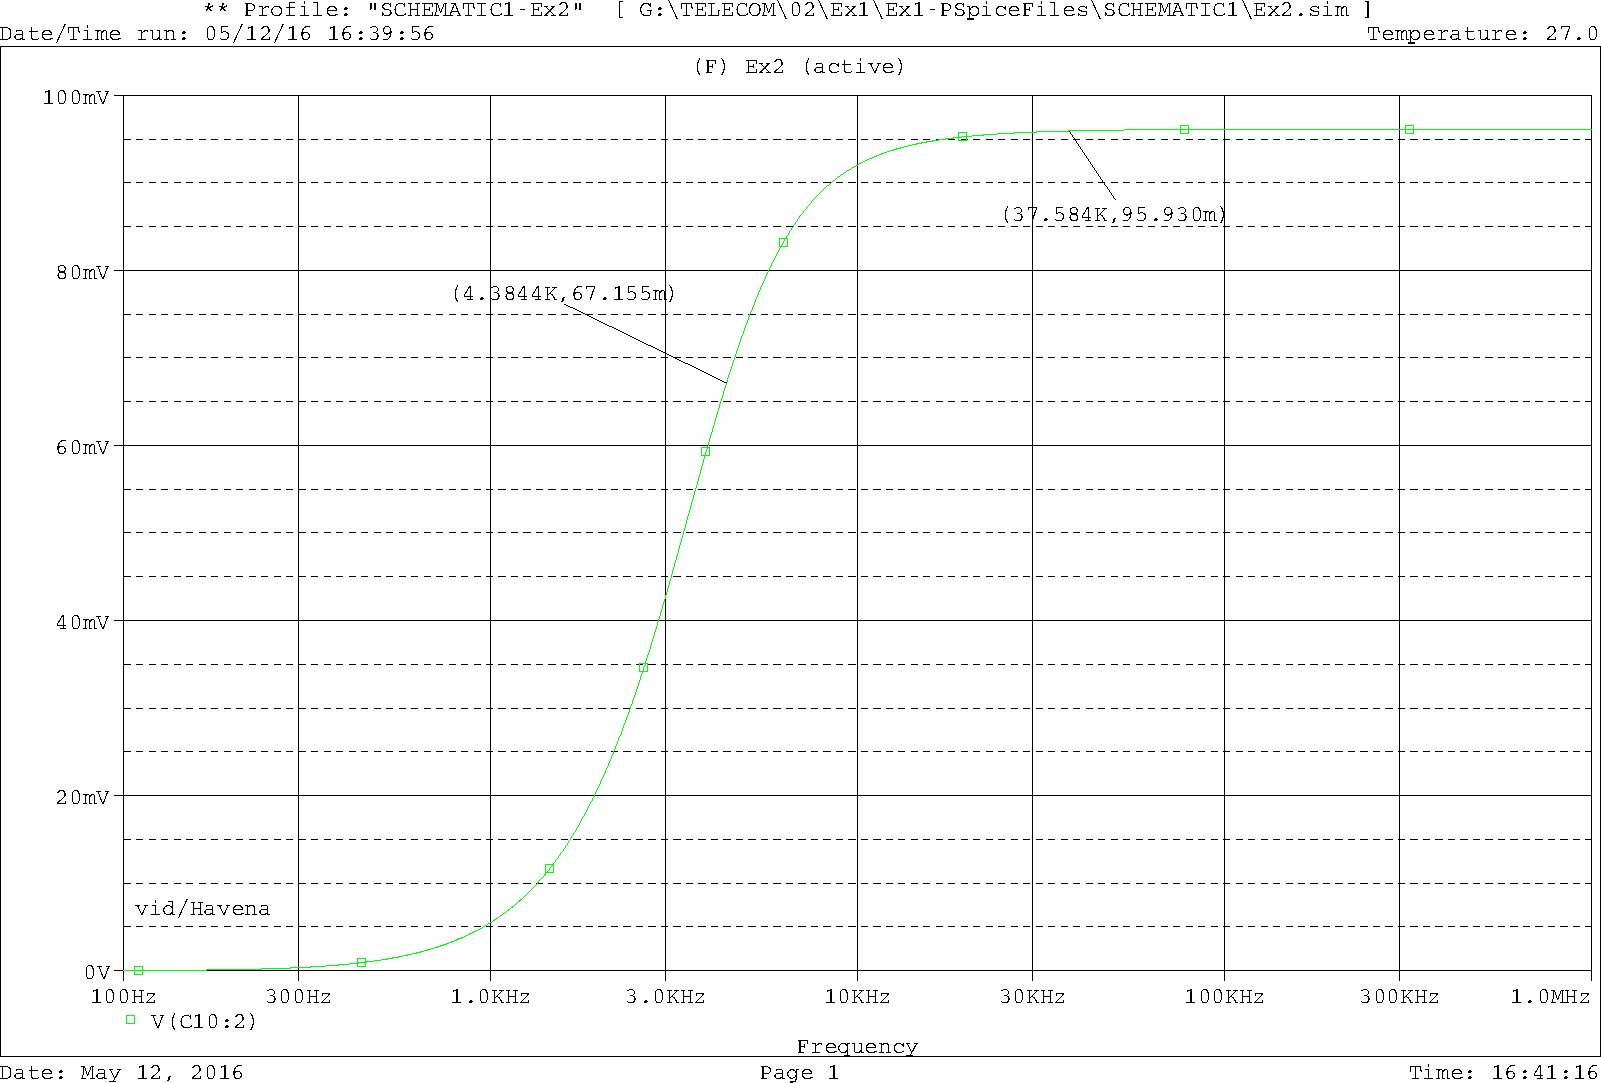
\includegraphics[scale=0.3]{Imagens/resp_freq_2}
  \label{fig:resp_freq_2}
  \caption{Resposta em frequência do filtro passa-altas.}
\end{figure}

A figura \ref{fig:resp_freq_db_2} mostra a resposta em dB, nota-se que a 
atenuação aumenta em aproximadamente 60 dB por década, o que corresponde a 
ordem 3 do filtro.

\begin{figure}[!h]
  \centering
  
  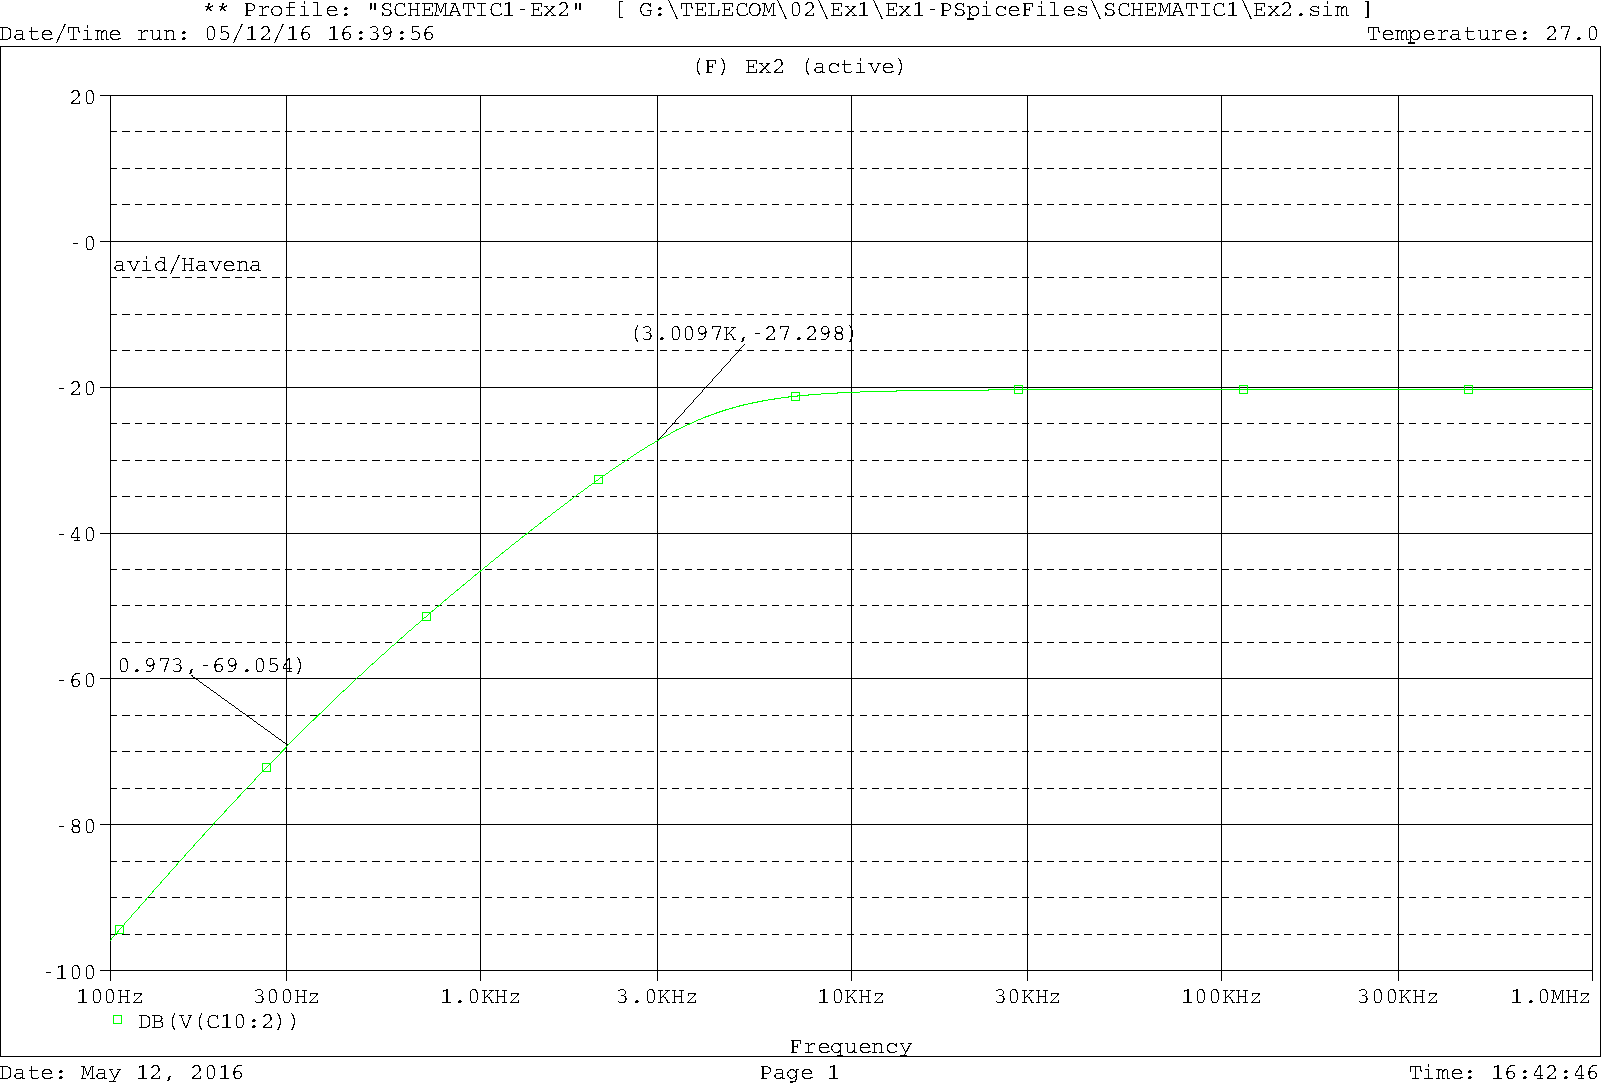
\includegraphics[scale=0.3]{Imagens/resp_freq_db_2}
  \label{fig:resp_freq_db_2}
  \caption{Resposta em frequência do filtro passa-altas em dB.}
\end{figure}

A figura \ref{fig:resp_freq_phase_2} mostra a fase da resposta em frequência 
para o filtro passa altas, onde é possível observar uma defasagem de 270 graus, 
o que condiz com a teoria pois o filtro é de ordem 3.

\begin{figure}[!h]
  \centering
  
  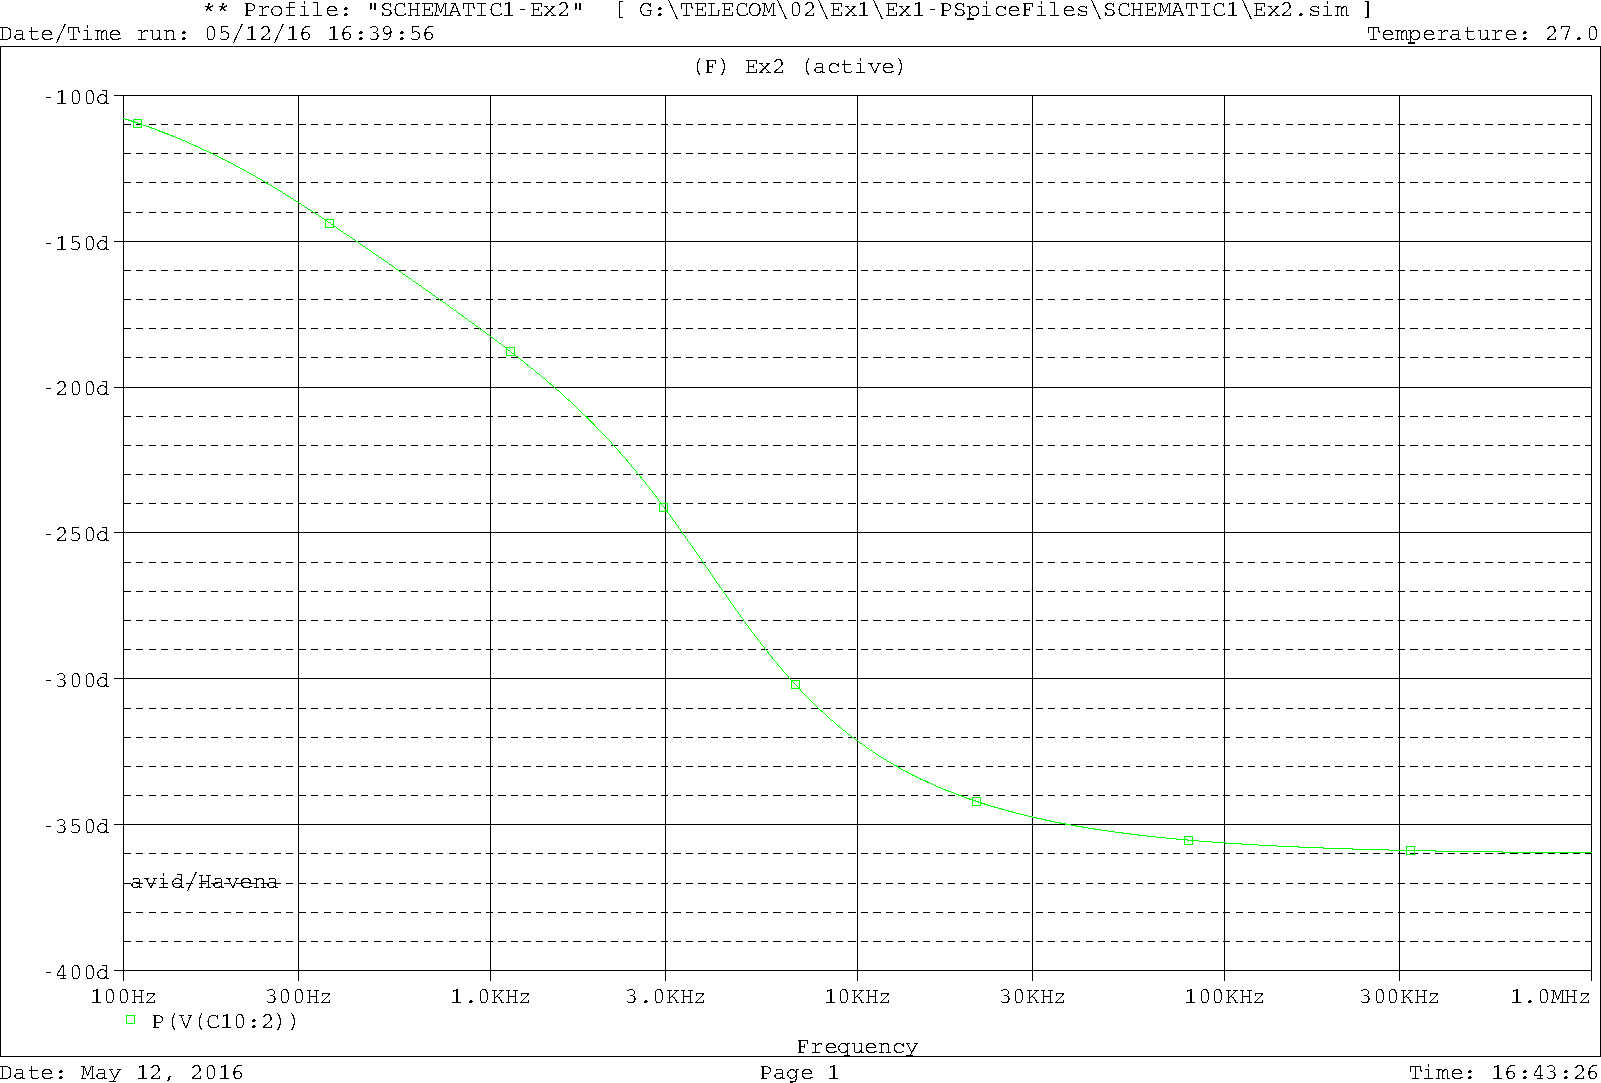
\includegraphics[scale=0.3]{Imagens/resp_freq_phase_2}
  \label{fig:resp_freq_phase_2}
  \caption{Fase da resposta em frequência do filtro passa-altas.}
\end{figure}

\subsection{FPF em cascata}
O terceiro filtro projetado foi um filtro passa-faixas em cascata de terceira 
ordem, com resposta do tipo Butterworth utilizando apenas 1 indutor.

A figura \ref{fig:fpf-cascata} mostra o circuito já desnormalizado, pronto para 
simulação.

\begin{figure}[!h]
  \centering
  
  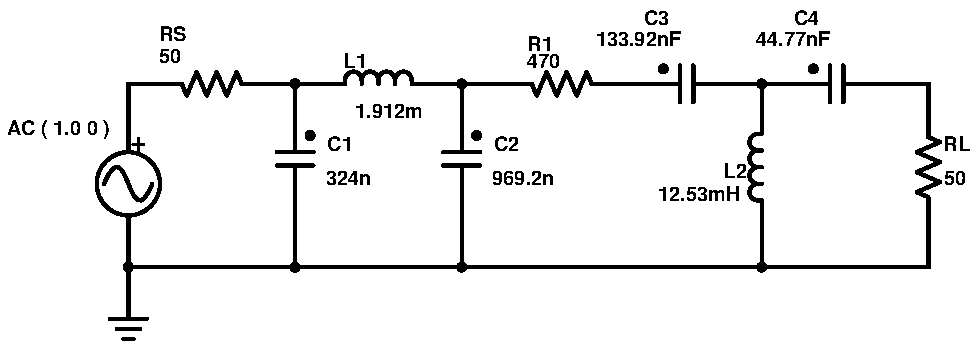
\includegraphics[scale=0.4]{Imagens/fpf-cascata}
  \label{fig:fpf-cascata}
  \caption{Filtro desnormalizado passa-faixa em cascata.}
\end{figure}

A resposta em frequência obtida está na figura \ref{fig:resp_freq_3}, onde foi 
obtido uma frequência central de 4,655 kHz. 

\begin{figure}[!h]
  \centering
  
  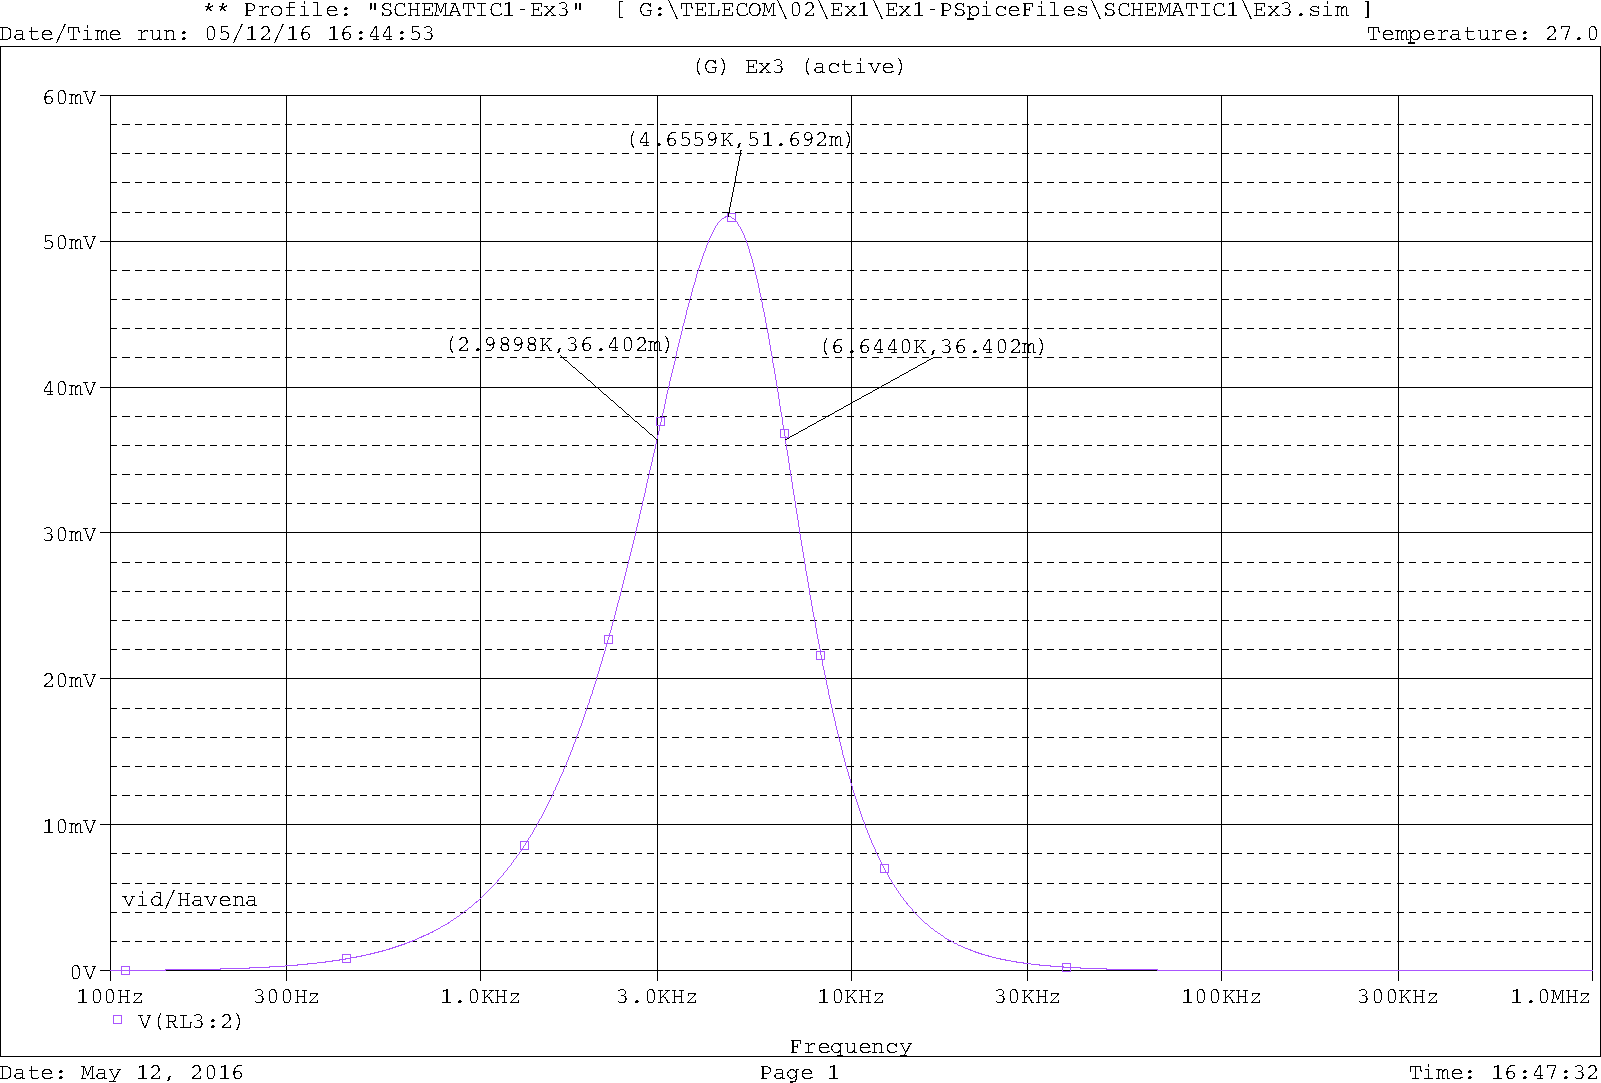
\includegraphics[scale=0.3]{Imagens/resp_freq_3}
  \label{fig:resp_freq_3}
  \caption{Resposta em frequência do filtro passa-faixa em cascata.}
\end{figure}

A figura \ref{fig:resp_freq_db_3} mostra a resposta em dB, nota-se que a 
atenuação aumenta em aproximadamente 60 dB por década, o que corresponde a 
ordem 3 do filtro.

\begin{figure}[!h]
  \centering
  
  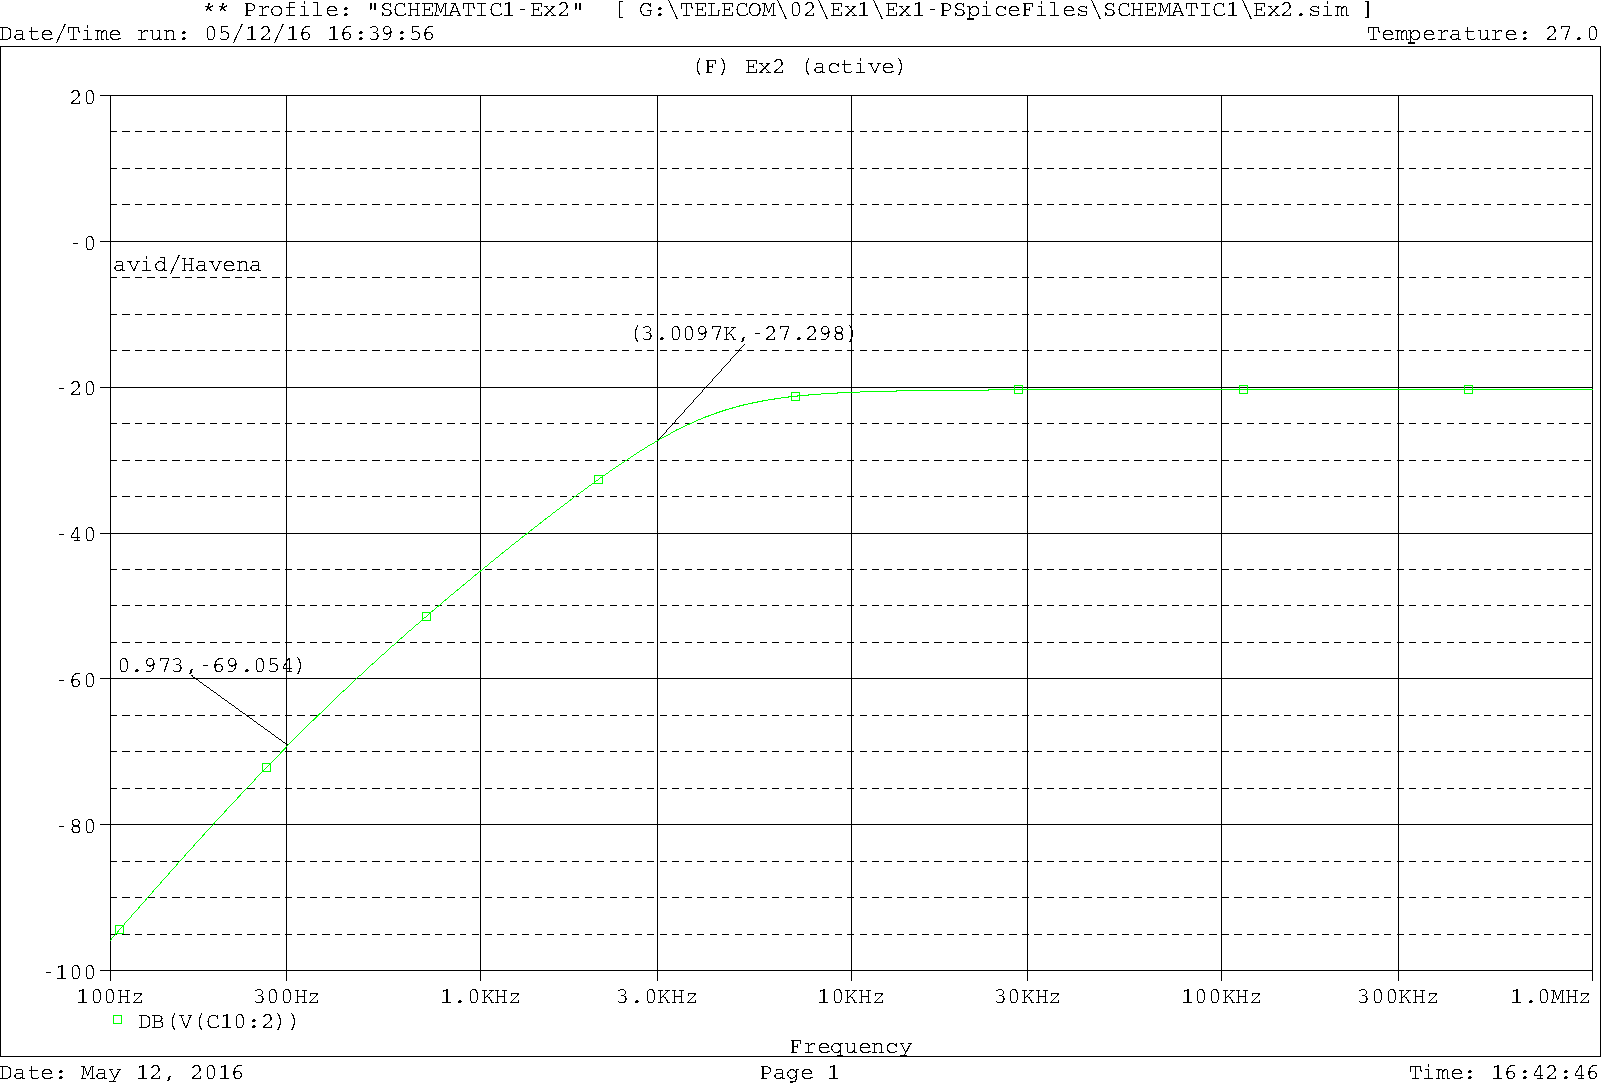
\includegraphics[scale=0.3]{Imagens/resp_freq_db_2}
  \label{fig:resp_freq_db_3}
  \caption{Resposta em frequência do filtro passa-faixa em cascata em dB.}
\end{figure}

A figura \ref{fig:resp_freq_phase_3} mostra a fase da resposta em frequência 
para o filtro passa altas, onde é possível observar uma defasagem de 270 graus, 
o que condiz com a teoria pois o filtro é de ordem 3.

\begin{figure}[!h]
  \centering
  
  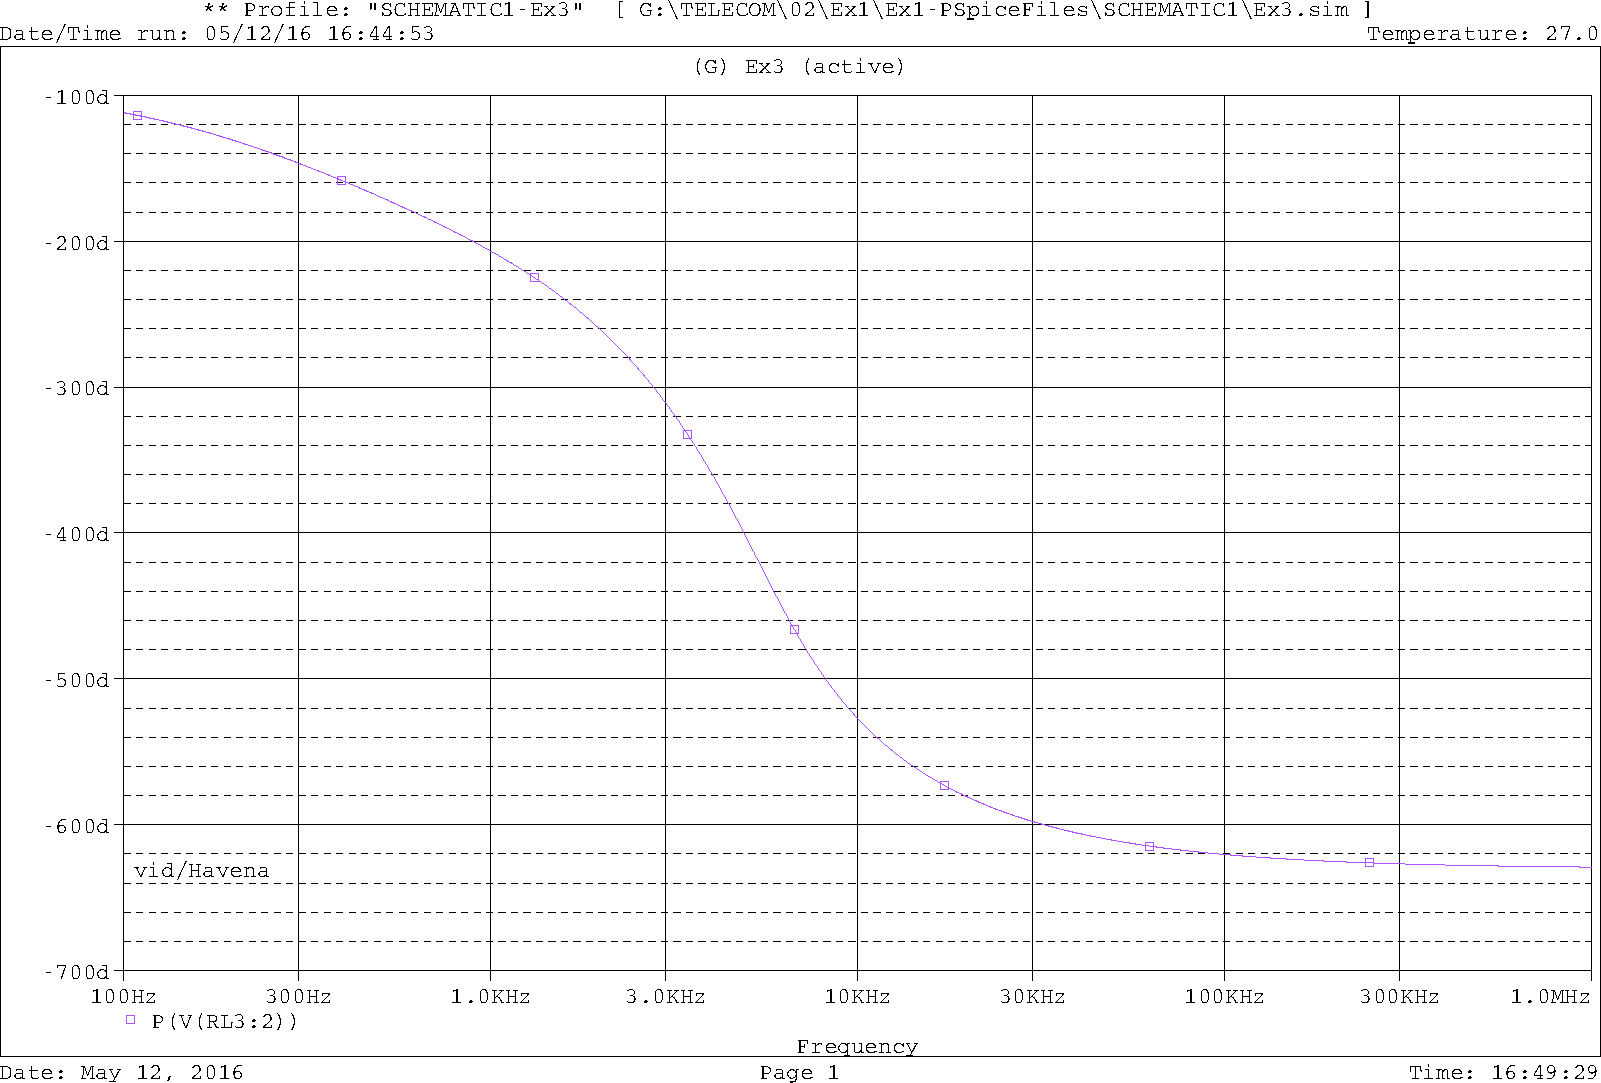
\includegraphics[scale=0.3]{Imagens/resp_freq_phase_3}
  \label{fig:resp_freq_phase_3}
  \caption{Fase da resposta em frequência do filtro passa-faixa em cascata.}
\end{figure}

\subsection{FPF}
O quarto e ultimo filtro foi projetado para ter uma resposta em frequência 
semelhante a do filtro FPF. O objetivo foi de analisar as diferenças 
em se utilizar um filtro FPF e um filtro FPB em conjunto com um filtro FPA.

O terceiro filtro projetado foi um filtro passa-faixas em cascata de terceira 
ordem, com resposta do tipo Butterworth utilizando apenas 1 indutor.

A figura \ref{fig:fpf} mostra o circuito já desnormalizado, pronto para 
simulação.

\begin{figure}[!h]
  \centering
  
  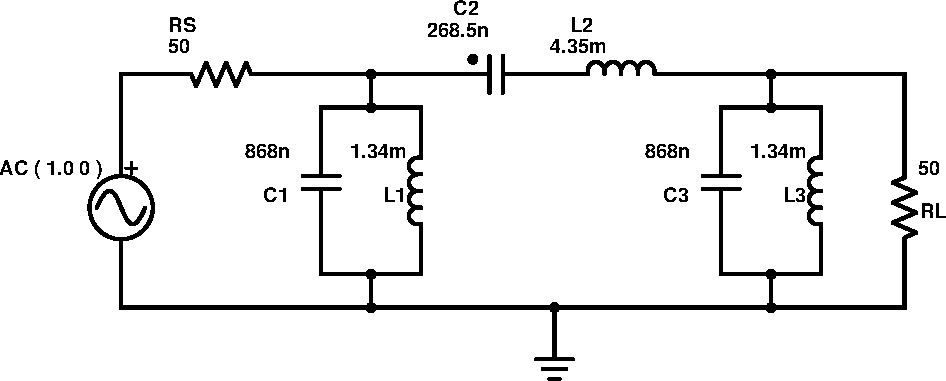
\includegraphics[scale=0.4]{Imagens/fpf}
  \label{fig:fpf}
  \caption{Filtro desnormalizado passa-faixa.}
\end{figure}

A resposta em frequência obtida está na figura \ref{fig:resp_freq_4}, onde foi 
obtido uma frequência central de 4,655 kHz. 

\begin{figure}[!h]
  \centering
  
  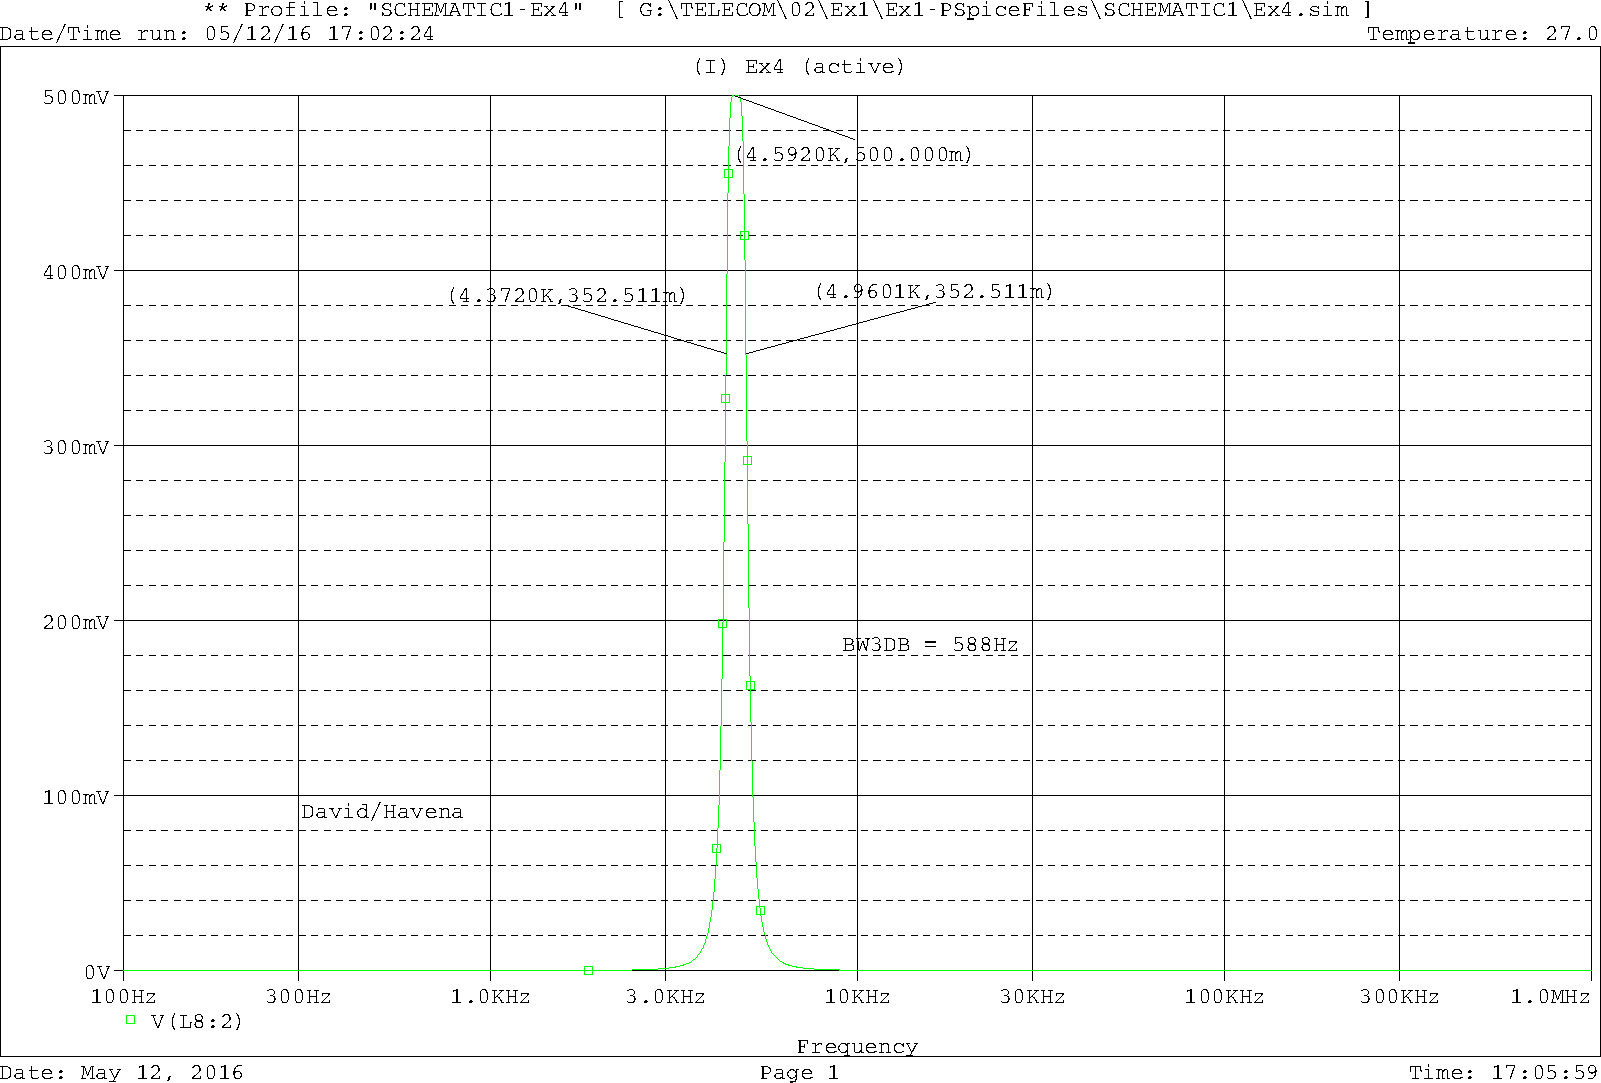
\includegraphics[scale=0.3]{Imagens/resp_freq_4}
  \label{fig:resp_freq_4}
  \caption{Resposta em frequência do filtro passa-faixa.}
\end{figure}

A figura \ref{fig:resp_freq_db_4} mostra a resposta em dB, nota-se que a 
atenuação aumenta em aproximadamente 60 dB por década, o que corresponde a 
ordem 3 do filtro.

\begin{figure}[!h]
  \centering
  
  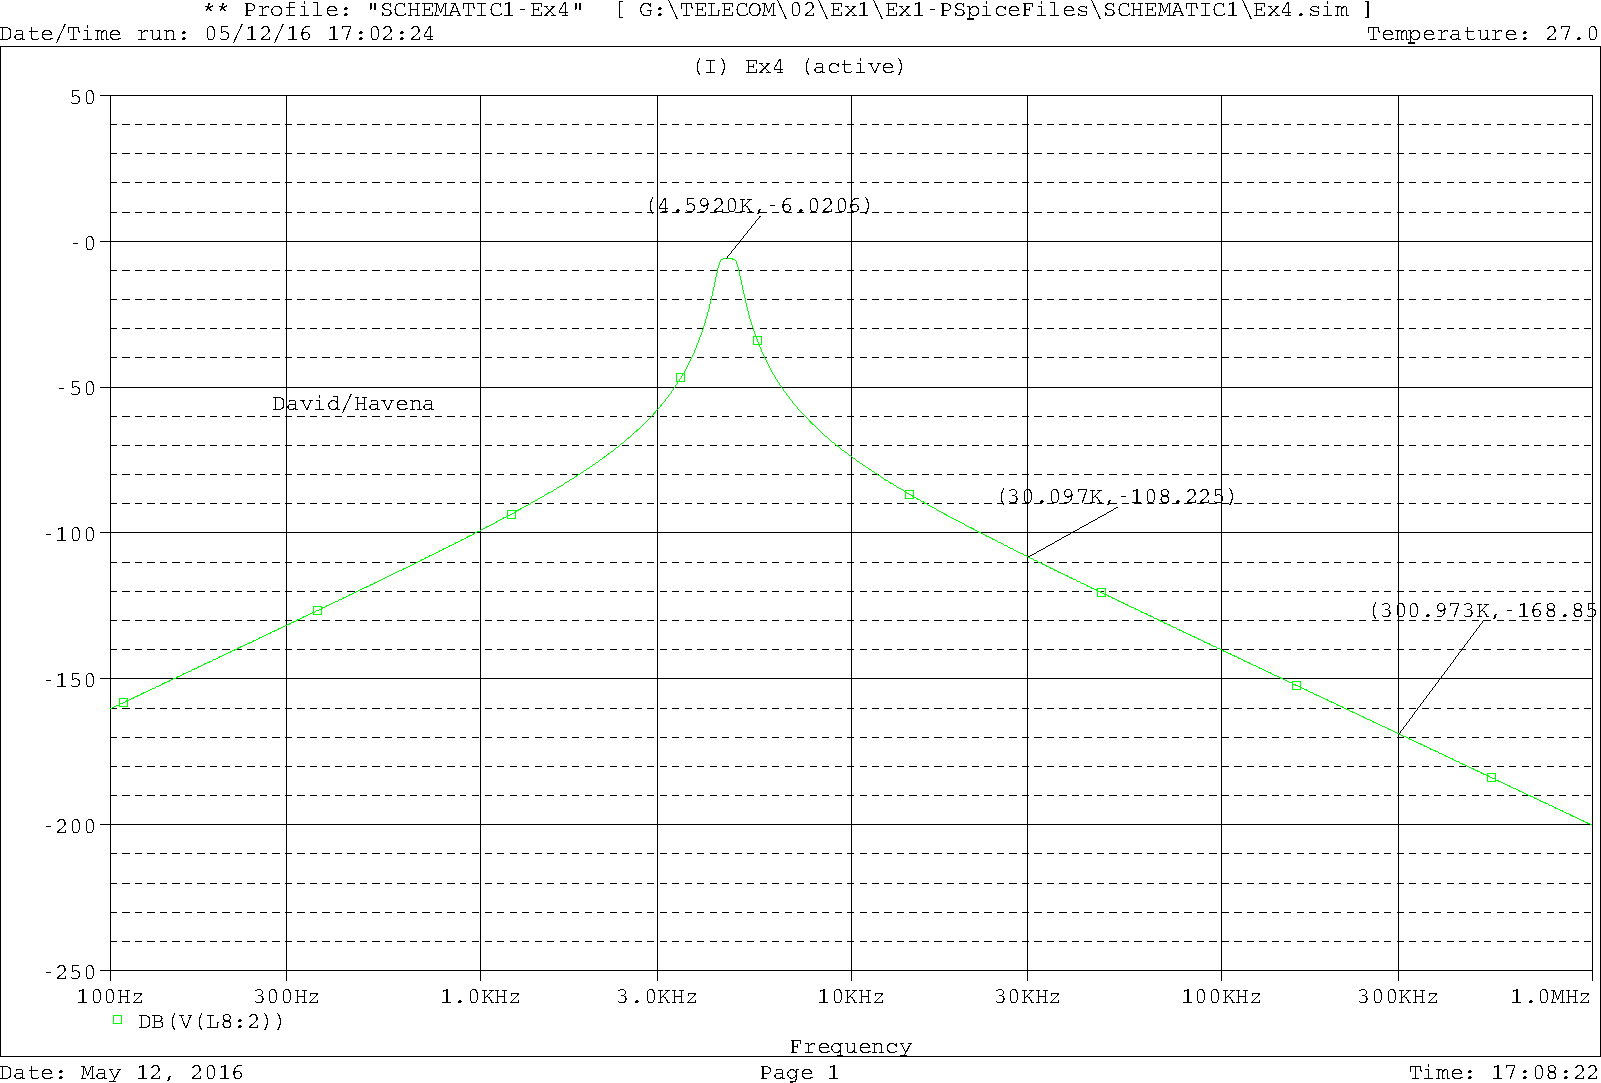
\includegraphics[scale=0.3]{Imagens/resp_freq_db_4}
  \label{fig:resp_freq_db_4}
  \caption{Resposta em frequência do filtro passa-faixa em dB.}
\end{figure}

A figura \ref{fig:resp_freq_phase_4} mostra a fase da resposta em frequência 
para o filtro passa altas, onde é possível observar uma defasagem de 270 graus, 
o que condiz com a teoria pois o filtro é de ordem 3.

\begin{figure}[!h]
  \centering
  
  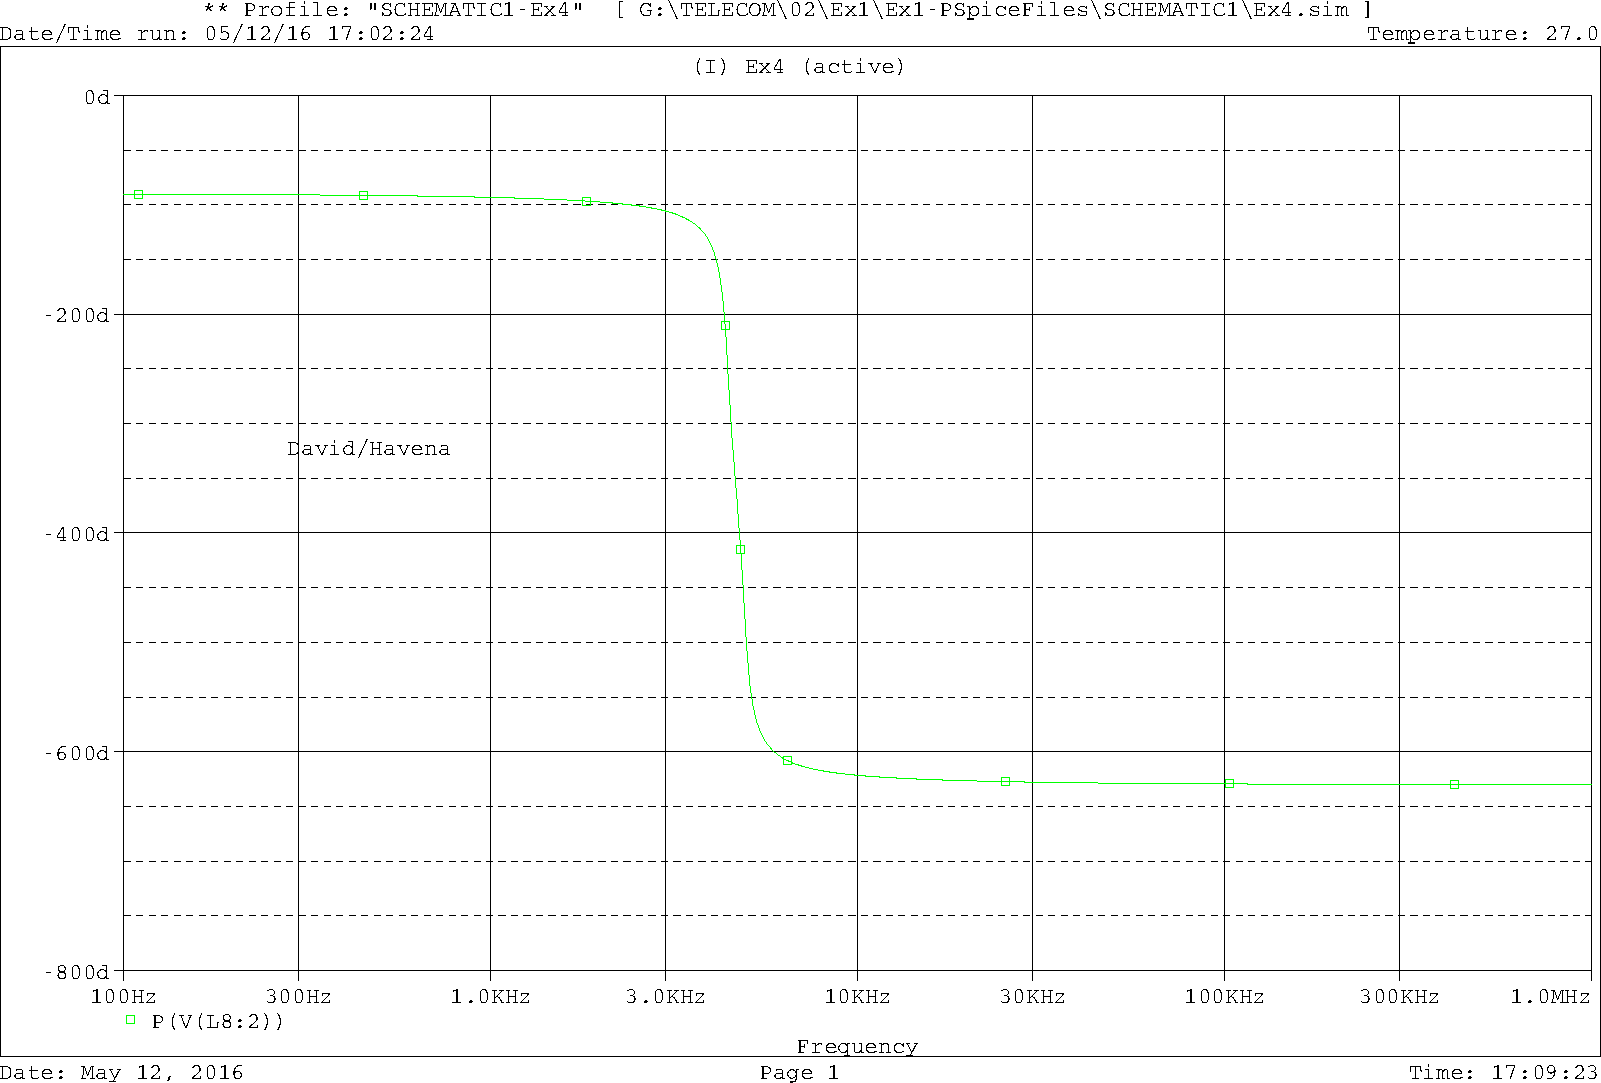
\includegraphics[scale=0.3]{Imagens/resp_freq_phase_4}
  \label{fig:resp_freq_phase_4}
  \caption{Fase da resposta em frequência do filtro passa-faixa.}
\end{figure}